%!TEX root = ../terrainbook.tex


\graphicspath{{runoff/}}
% \setchapterpreamble[u]{\margintoc}
\setchapterpreamble[u]{\youtube[0pt]{youtu.be/0NzZoJATFjc}\margintoc[18pt]}




\chapter{Runoff modelling}%
\label{chap:runoff}

Many interesting DTM operations are based on runoff modelling, \ie\ the computation of the flow and accumulation of water on a terrain.
Examples include: knowing where streams will form in the case of heavy rainfall, finding the areas that will be affected by a waterborne pollutant, tracing the areas that could become submerged by floodwater, or calculating the rate of erosion or sedimentation in a given area.

In hydrology, runoff modelling can be very complex (Figure~\ref{fig:hydrology}).
Hydrological models usually consider different precipitation scenarios, model various types of overland and subsurface flows, and take into account many location- and time-dependent factors, such as the depth of the water table and the permeability of the soil.
Such models can be quite accurate, but they require high-resolution data that is often not available, they are difficult to create without specialised knowledge, and they involve substantial manual work.

\begin{figure}
\centering
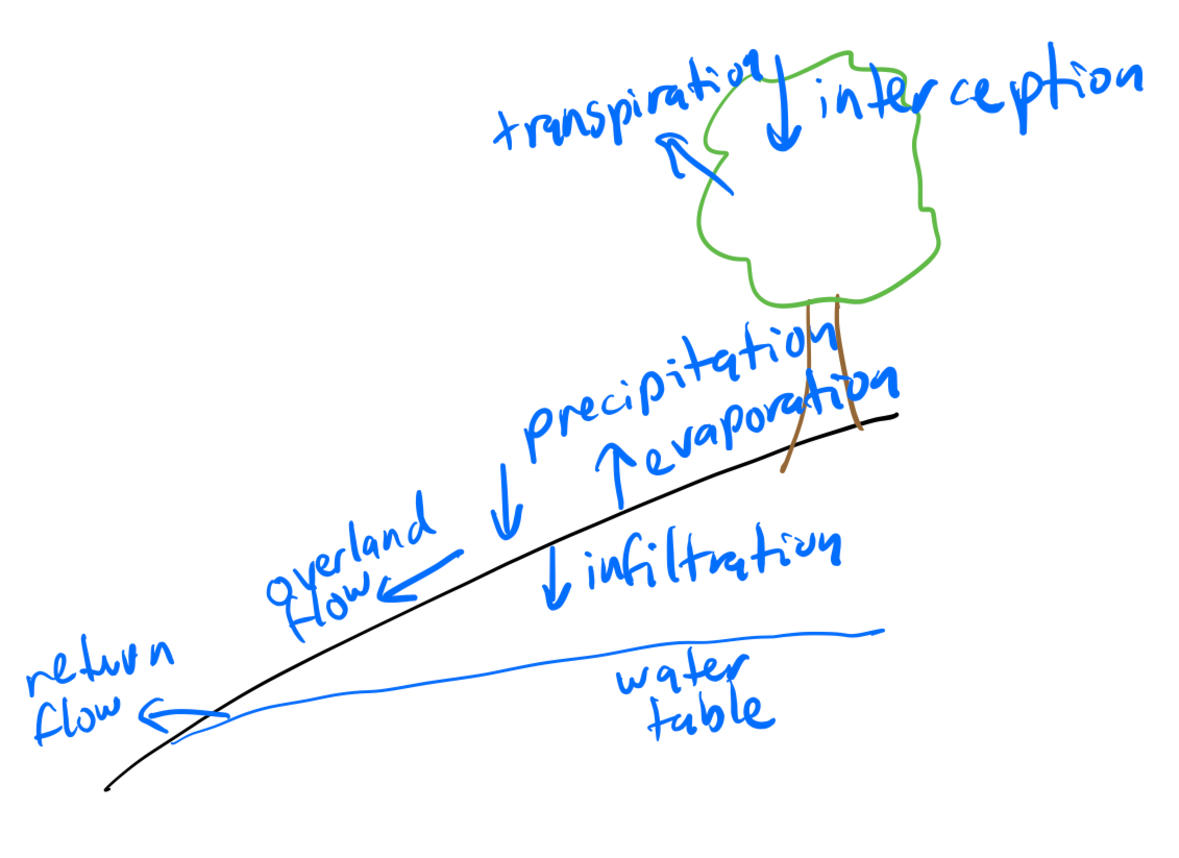
\includegraphics[width=0.95\linewidth]{figs/hydrology.pdf}
\caption{Different types of water flows as modelled in hydrology. Figure adapted from \citet{Beven12}.}%
\label{fig:hydrology}
\end{figure}

By contrast, the simpler \emph{GIS models of runoff} can be performed automatically in large areas with only a DTM\@.
These models mostly use gridded raster terrains, and so we will generally refer to these in this chapter, but the methods described here mostly work just as well with other representations (\eg\ a TIN).
In order for the GIS models of runoff to achieve their results, two big assumptions are usually made:

\begin{enumerate}
\item that all water flow is \emph{overland}, thus ignoring all subsurface flows and dismissing factors such as evaporation and infiltration; and
\item that a good estimate for the total flow at any point is the drainage area upstream from it, \ie\ the area above the point which drains through/to it, which is roughly equivalent to rain that is falling evenly all over a terrain.
\end{enumerate}

Based on these assumptions, runoff modelling is simplified by considering only two values, which are computed for every cell in a DTM\@:

\begin{description}
\item[Flow direction]
Given\marginnote{flow direction}\index{flow direction} a DTM cell, towards which nearby cells and in which proportions does water flow from it?
\item[Flow accumulation]
Given\marginnote{flow accumulation}\index{flow accumulation} a DTM cell, what is the total water flow that passes through it?
\end{description}

We look at a few different methods to compute these values in the next two sections.

\section{Computing the flow direction}[Flow direction]%
\label{se:direction}

Theoretically, the flow direction of a point is the direction with the steepest descent at that location, which does correspond to the direction towards which water would naturally flow.
However, the discretisation of a terrain into DTM cells means that some kind of an approximation needs to be made.
There are two broad approaches that can be followed to do this: computing a single flow direction, which assumes that all the water in a DTM cell flows to one other cell, or multiple flow directions, which assumes that the water in a DTM cell can flow towards multiple other cells.

\subsection{Single flow direction}

% Perpendicular to contours in a 2D map

The earliest and simplest method to compute the flow direction of a cell is to compute the slope between the centre of the cell and the centre of all its neighbouring cells (using the distance between the centres and the difference in elevation), then assign the flow direction towards the neighbour with the steepest descent.
The method is known as the \emph{single flow direction (SFD)}\marginnote{single flow direction (SFD)}\index{single flow direction}\index{SFD} approach, 
and when applied to a raster grid, it usually considers that there are eight neighbours to each pixel (left, right, up, down and the diagonals).
For this reason, it is also known as the \emph{eight flow directions (D8)}\marginnote{D8 flow direction}\index{D8 flow direction}\index{eight flow directions} approach.

On one hand, the method is very fast and easy to implement, and it avoids dispersing the water flow between multiple cells.
On the other hand, it can have significant errors in the flow direction, and it does not allow for divergent flows.
For instance, in a square grid, the errors can be of up to \(22.5^\circ{}\) (because the method is forced to choose a neighbouring cell in increments of \(45^\circ{}\)).
This method can therefore easily create artefacts in certain geometric configurations (Figure~\ref{fig:d8}).

\begin{figure}[htbp]
\centering
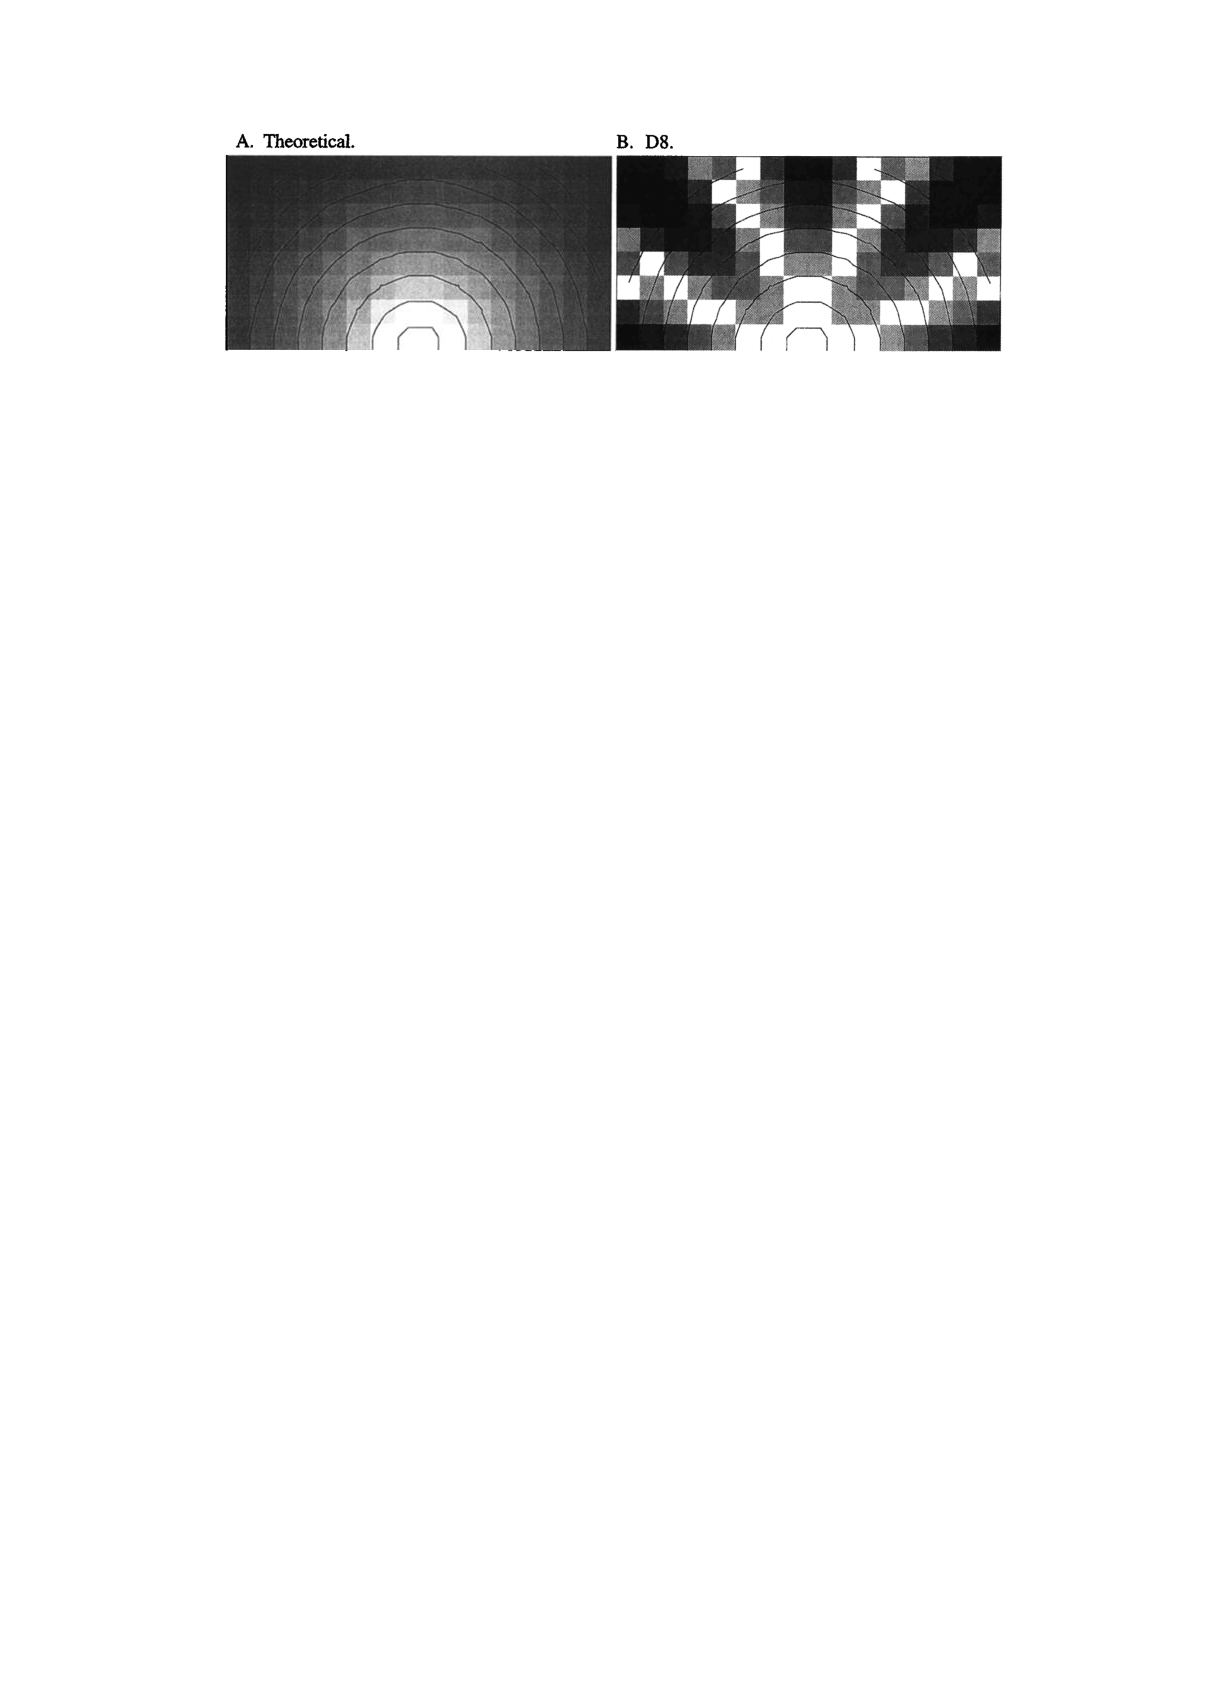
\includegraphics[width=0.95\linewidth]{figs/d8.pdf}
\caption{The D8 method creates artefacts when water is draining from a circular cone. Figure from \citet{Tarborton97}.}%
\label{fig:d8}
\end{figure}

Many of these artefacts can be eliminated by using the rho8 (\(\rho8\))\marginnote{rho8 (\(\rho8\))}\index{\(\rho8\)}\index{rho8} method, which modifies D8 to assign the flow direction to one of its lower neighbours randomly with probability proportional to the slope.
However, it produces non-deterministic results, which is often a sufficient reason not to use it.

Despite its age and limitations, the SFD method is still widely used and available in many GIS tools\@.

\subsection{Multiple flow directions}

In an attempt to overcome the limitations of the SFD method, a variety of methods assign the flow direction of a DTM cell fractionally to some or all of its lower neighbouring cells according to some criteria.
These methods are collectively known as multiple flow directions (MFD), 
\marginnote{multiple flow directions (MFD)}\index{multiple flow directions}\index{MFD}
and they usually use a variation of this equation:

\begin{equation}
F_i = \frac{\left(L_i \tan{\alpha_i}\right)^x}{\sum_{j=1}^{n}\left(L_j \tan{\alpha_j}\right)^x}
\end{equation}

where \(F_i\) is the flow towards the i-th neighbouring cell, \(L_i\) is the flow width (Figure~\ref{fig:quinn}), \(\alpha_i\) is the gradient towards the i-th neighbouring cell (and so \(\tan(\alpha_i)\) is the slope), \(x\) is an exponent that controls the dispersion, and \(n\) is the number of neighbours of the cell.

\begin{marginfigure}
\centering
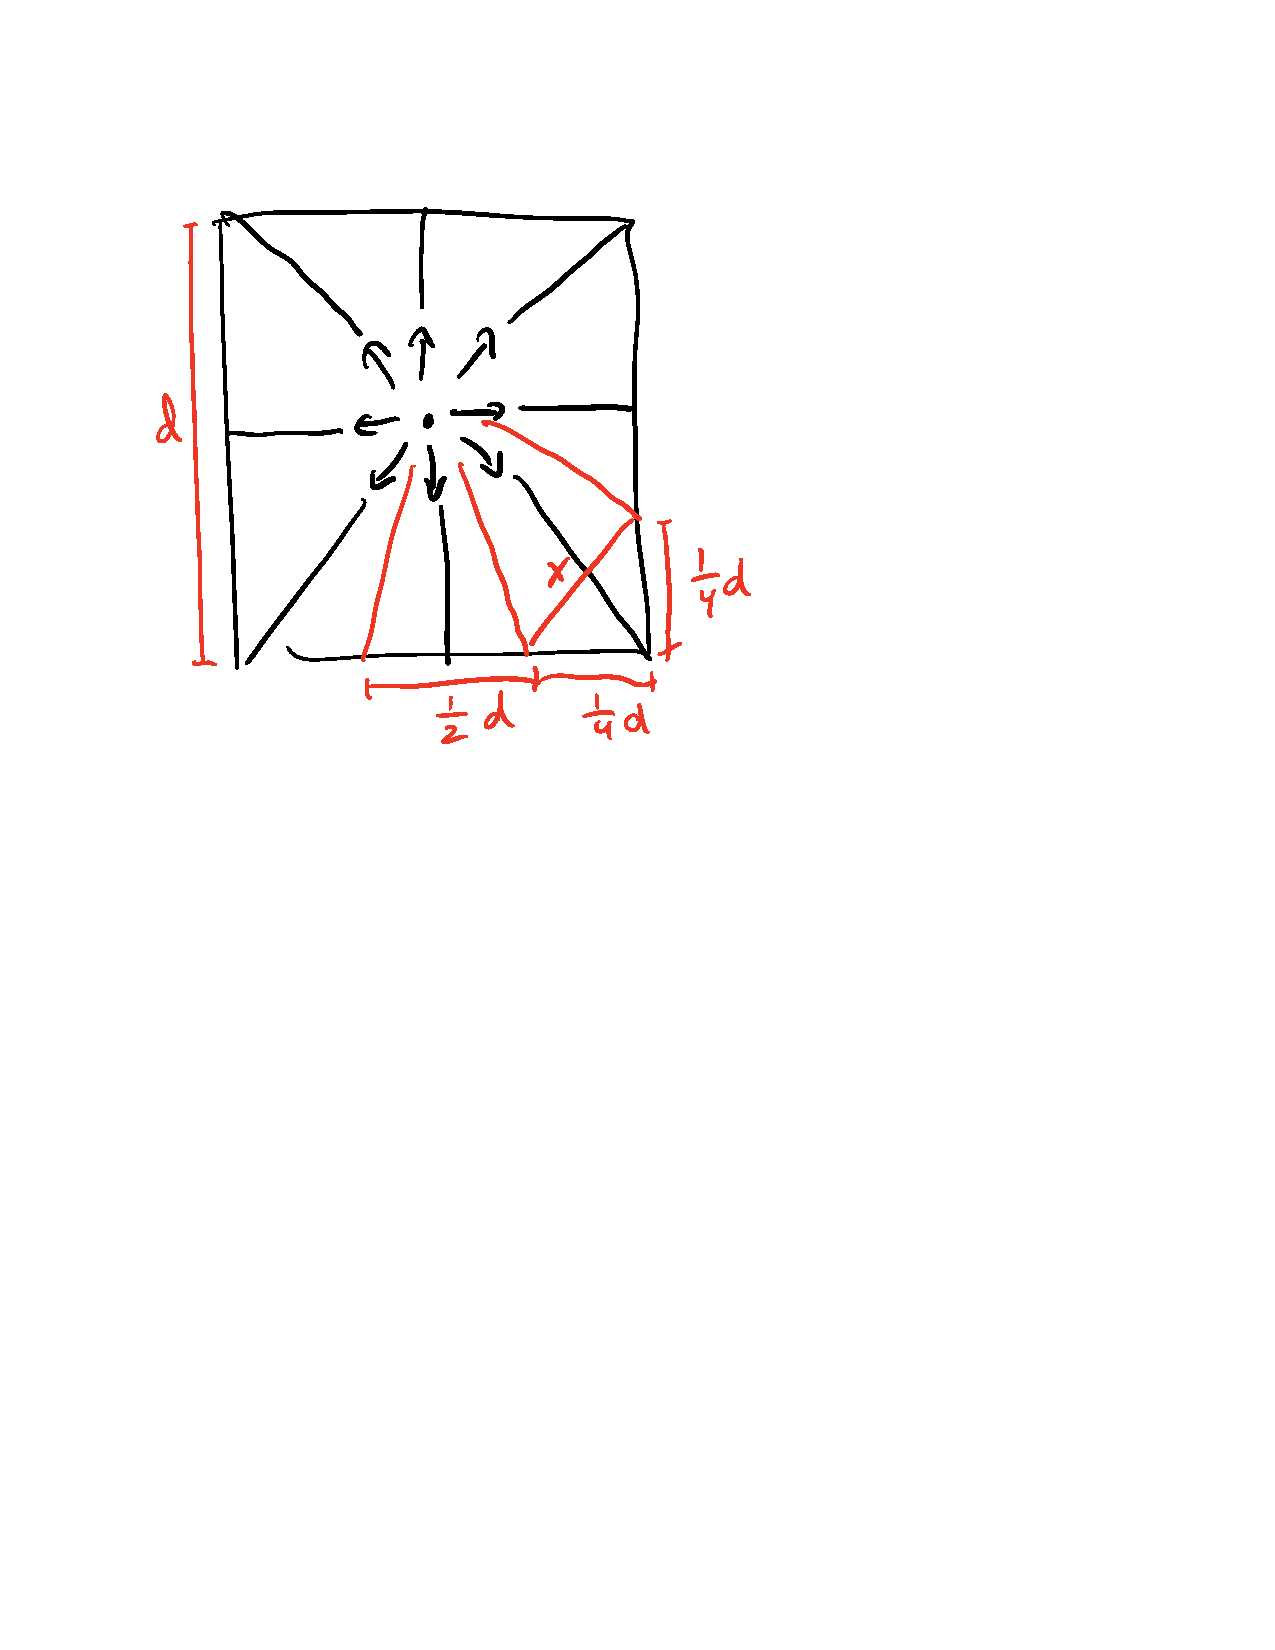
\includegraphics[width=\linewidth]{figs/quinn.pdf}
\caption{The flow width \(L\) can be computed using the geometry of the DTM cells.
In the case of a square grid with spacing \(d\), it is \(\frac{\sqrt{2}}{4}d\) for the diagonals (\(L_2\)) and \(\frac{1}{2}d\) for the adjacencies (\(L_1\)), where \(d\) is the grid spacing. Based on \citet{Quinn91}.}%
\label{fig:quinn}
\end{marginfigure}

As shown in Figure~\ref{fig:dispersion}, MFD methods show characteristically wider flows compared to SFD methods.
D8 does not disperse the flow, but the path is constrained to the 8 possible grid directions.
By contrast, \citet{Quinn91} (an MFD method) can model the flow direction in a way that matches the topography better, but it also introduces substantial dispersion.
More modern approaches try to combine some of the advantages of both approaches.

\begin{figure}[htbp]
\centering
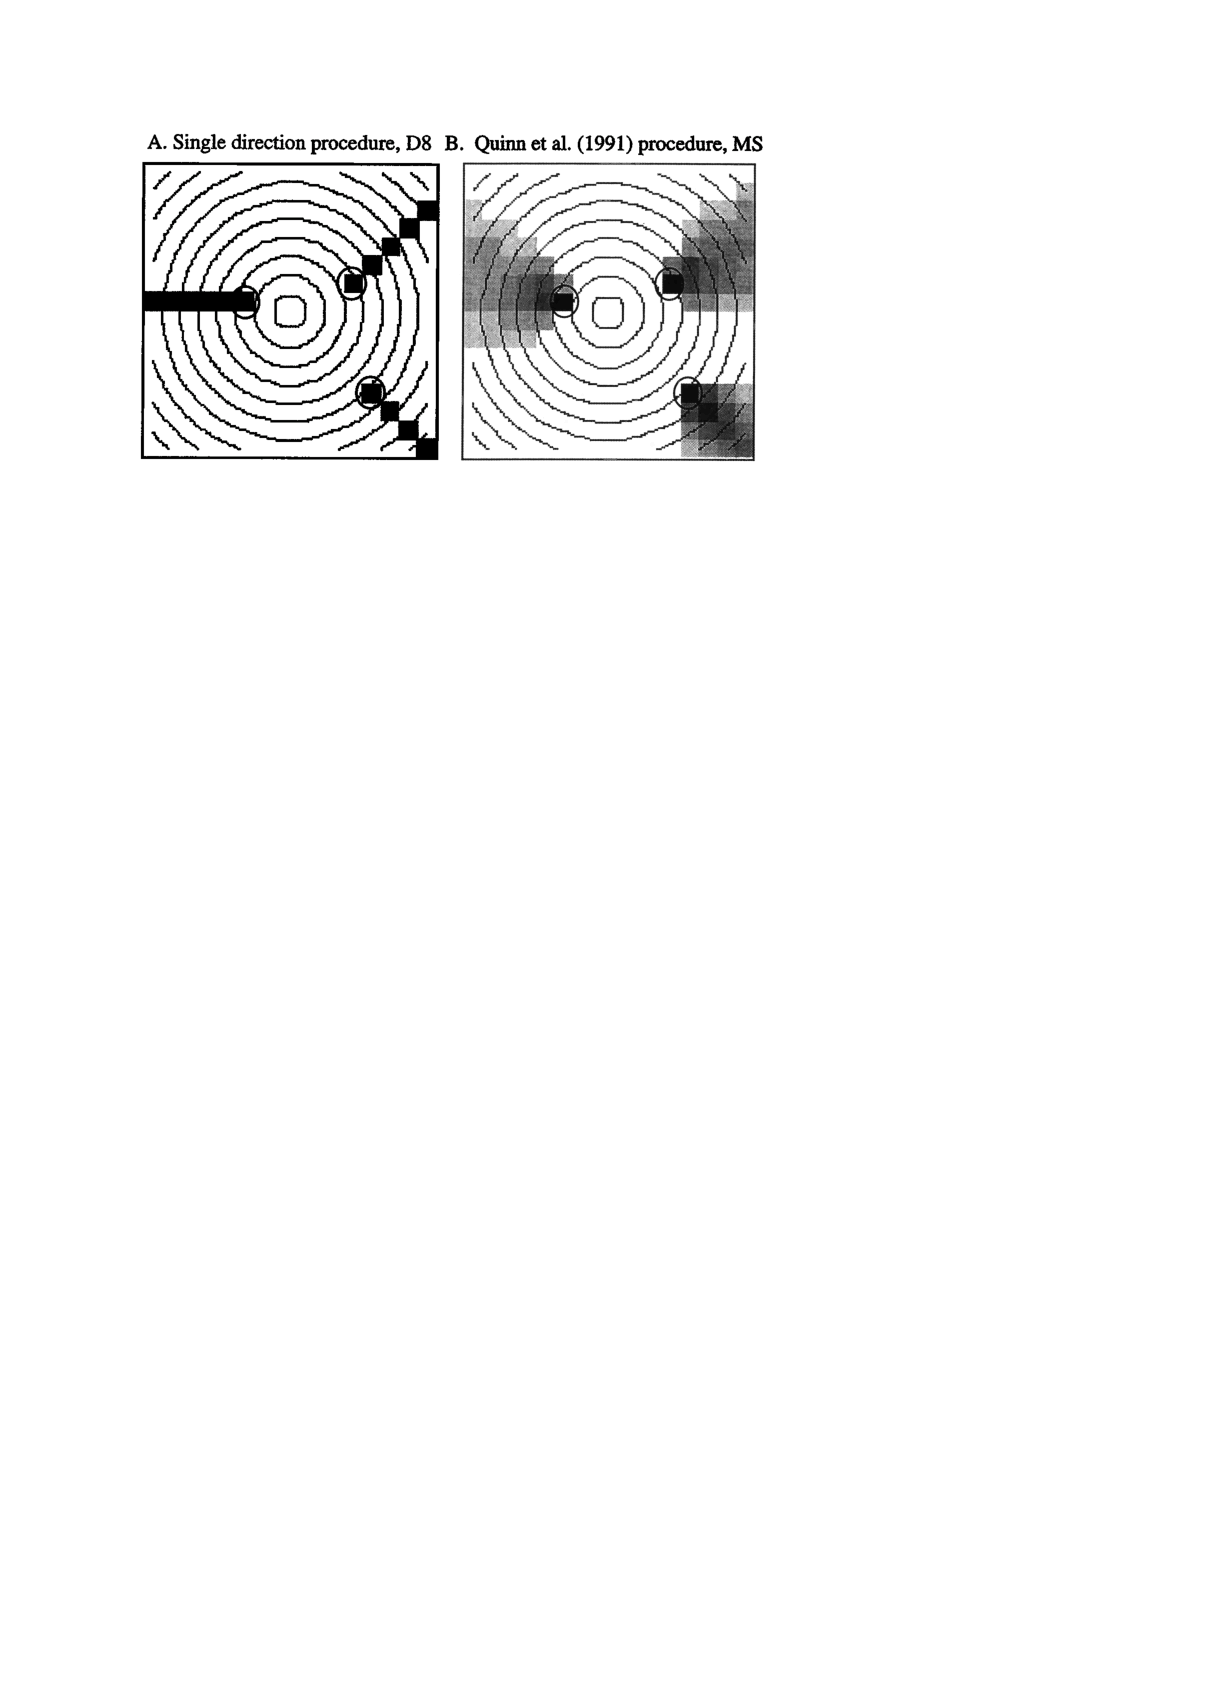
\includegraphics[width=0.95\linewidth]{figs/dispersion.pdf}
\caption{Flows in a circular cone: SFD (D8) vs.\ MFD\@ (\citet{Quinn91}). Figure from \citet{Tarborton97}.}%
\label{fig:dispersion}
\end{figure}

\section{Computing the flow accumulation}[Flow accumulation]%
\label{se:accumulation}

After the flow directions in all the cells of a DTM have been computed, the usual next step is to use this information to compute the flow accumulation in all of them.
As stated in the assumptions we make for GIS models of runoff, the flow accumulation at a given DTM cell can be estimated by the area that drains to it.
Note that in the case of a square grid, it is simply the number of cells that drain to it.

In practical terms, the flow accumulation is defined based on a recursive operation:

\begin{equation}
A_0 = a_0 + \sum_{i=1}^{n} p_i A_i
\end{equation}

where \(A_0\) is the accumulated flow for a cell, \(a_0\) is the area of the cell, \(p\) is the proportion of the i-th neighbour that drains to the cell, \(A_i\) is the accumulated flow for the i-th neighbour, \(n\) is the total number of the neighbouring cells.
Note that this calculation can be sped up substantially by: (i) storing the accumulated flows that have already been computed, and (ii) not following the recursion when \(p_i = 0\).


%%%
\section{Solving issues with sinks}

\emph{Sinks}\marginnote{sink}\index{sink}, which are also known as depressions or pits, are areas in a DTM that are completely surrounded by higher terrain.
Some of these are natural features that are present in the terrain (\eg\ lakes and dry lakebeds) and where water would flow towards (and stagnate) in reality, and are thus not a problem for runoff modelling.
However, they can also be artefacts of the DTM (\eg\ noise and areas without vegetation can create depressions), or they can be very small areas that easily filled (\ie\ flooded), after which water would flow out of them.
In the latter case, we need to implement a mechanism to route water flows out of these depressions, since otherwise our runoff model could have very large water flows stopping at even tiny depressions.
We will look at two common options to solve this problem: modifying a DTM by filling in (certain) sinks, and implementing a flow routing algorithm that allows water to flow out of sinks.

\subsection{Filling in sinks}%
\index{sink filling}

The aim of the algorithms to fill in sinks is to increase the elevation of certain DTM cells in a way that ensures that all the cells in the DTM can drain to a cell on its boundary (Figure~\ref{fig:pf}), or possibly to a set of cells that are known to be valid outlets, \eg\ lakes and oceans\@.
At the same time, the elevation increases should be minimised in order to preserve the original DTM as much as possible.
In the best case scenario, we can imagine that the resulting DTM is one that resembles follows the terrain elevation of terrain where there is no water and the top of natural water bodies (but no artificial features as in a DEM).

\begin{figure}[htbp]
\centering
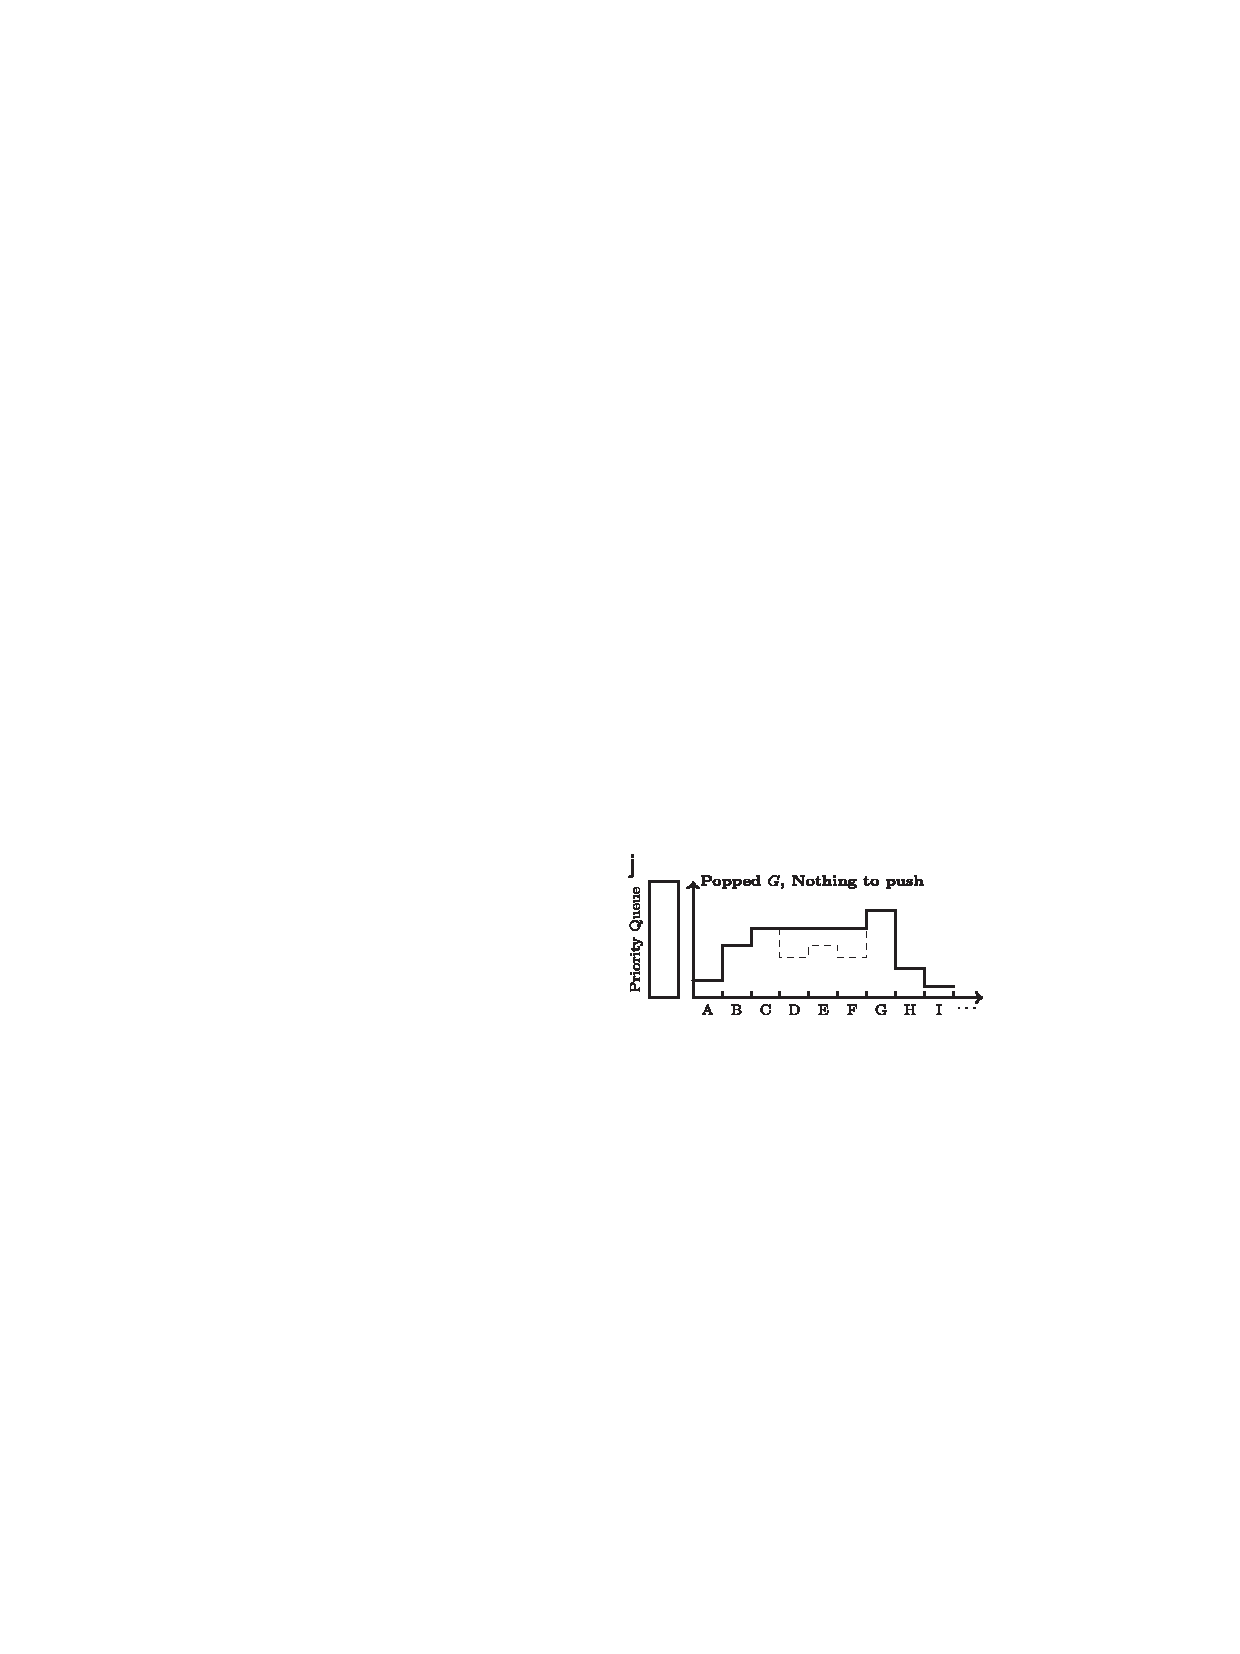
\includegraphics[width=0.8\linewidth]{figs/pf.pdf}
\caption{A vertical cross-section of a DTM with filled sinks. The dashed line represents the original terrain, whereas the thicker solid line represents the filled terrain. From \citet{Barnes14a}.}%
\label{fig:pf}
\end{figure}

One efficient method to fill in sinks is the priority-flood algorithm~\citep{Barnes14a}.
It works by keeping: (i) a list of DTM cells that are known to drain, which is kept sorted by elevation; and (ii) a raster marking whether each cell of the DTM is known to drain yet.
The list is initialised with the cells on the boundary of the DTM (which are assumed to be able to drain outwards), as well as other specially marked cells (\eg\ those forming part of a lake or a large river)\@.
Then, it iteratively: (i) removes the lowest cell from the sorted list of cells that are known to drain, (ii) increases the elevation of its neighbours that are not yet known to drain to the level of the cell, (iii) adds the neighbours that are not yet known to drain to the list.
Note that implicit in this last step is the fact that the neighbour cells are deemed to be able to drain through the current (lowest) cell.

\subsection{Least-cost (drainage) paths}

An alternative to modifying a DTM to eliminate sinks is to implement a more complex water routing algorithm that allows water to flow out of sinks.
For this, the usual approach is to implement a variation of the \(A^{*}\) search algorithm, which in this context is known as the least-cost paths (LCP)\marginnote{least-cost paths (LCP)}\index{least-cost paths}\index{LCP} algorithm~\citep{Metz11}.

The LCP algorithm is similar to priority-flood in that it keeps a sorted list of DTM cells that are known to drain, which is also initialised to the boundary pixels (and possibly other cells).
Then, it iteratively: (i) removes the lowest cell from this list, (ii) sets the drainage direction of its neighbours that are not yet known to drain towards itself, (iii) adds the neighbours that are not yet known to drain to the list.

\section{Assigning flow direction in flats}[Flow direction in flats]

\emph{Flats} are areas in a DTM that have the same elevation.
\marginnote{flat}\index{flat}
They therefore do not have a well-defined flow direction, which causes problems for many water routing algorithms.
Flats can sometimes occur naturally, but they are more often the result of precision limits, noise removal, or sink filling algorithms.

It is thus often necessary to apply a method that assigns a flow direction to flats, either by: (i) modifying the DTM to eliminate them, and then assigning them a flow direction in the usual way, or (ii) assigning them a flow direction directly.

After all flats in a DTM have been identified and their extent is known, algorithms usually work by (i) assigning an artificial gradient away from higher terrain (Figure~\ref{fig:ht}), \ie\ terrain in a flat is assumed to become lower as we move farther away from its neighbouring higher terrain; and/or (ii) assigning an artificial gradient towards lower terrain (Figure~\ref{fig:lt}), \ie\ terrain in a flat is assumed to become lower as we move closer to its neighbouring lower terrain.
\citet{Barnes14} is a good example of an efficient method that combines both of these approaches, resulting in more natural flow directions and better results than would be possible with either approach individually.

\begin{figure}[htbp]
\centering
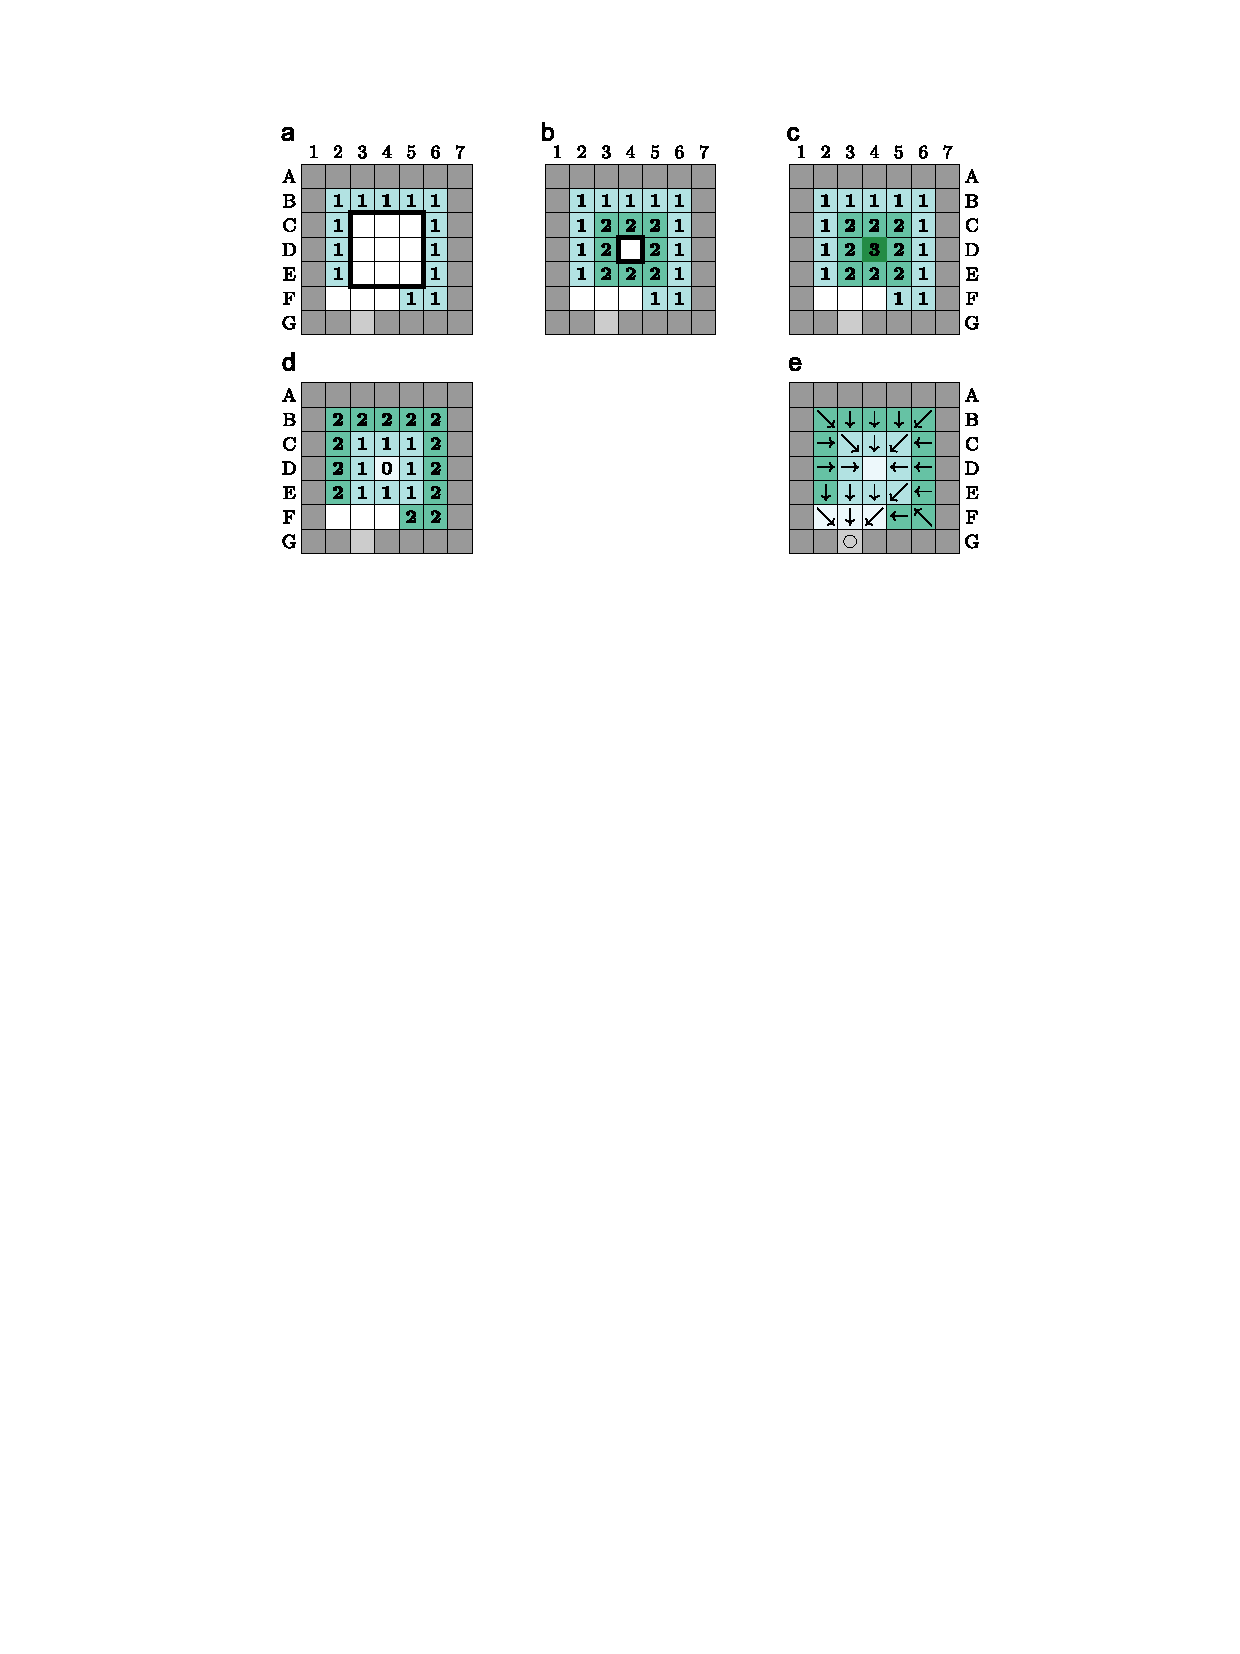
\includegraphics[width=1.0\linewidth]{figs/ht.pdf}
\caption{In a flat surrounded by higher terrain (dark grey) with a single lower-elevation outlet (light grey), we can use a gradient away from the higher terrain to route water out of the flat and towards the outlet.
For this, we can iteratively assign (tiny or symbolic) elevation decreases in the flat starting from the higher terrain until all non-draining cells in the flat have been covered.
Note that in this case, a sink is produced by the procedure.
Figure from \citet{Barnes14}.}%
\label{fig:ht}
\end{figure}

\begin{figure}[htbp]
\centering
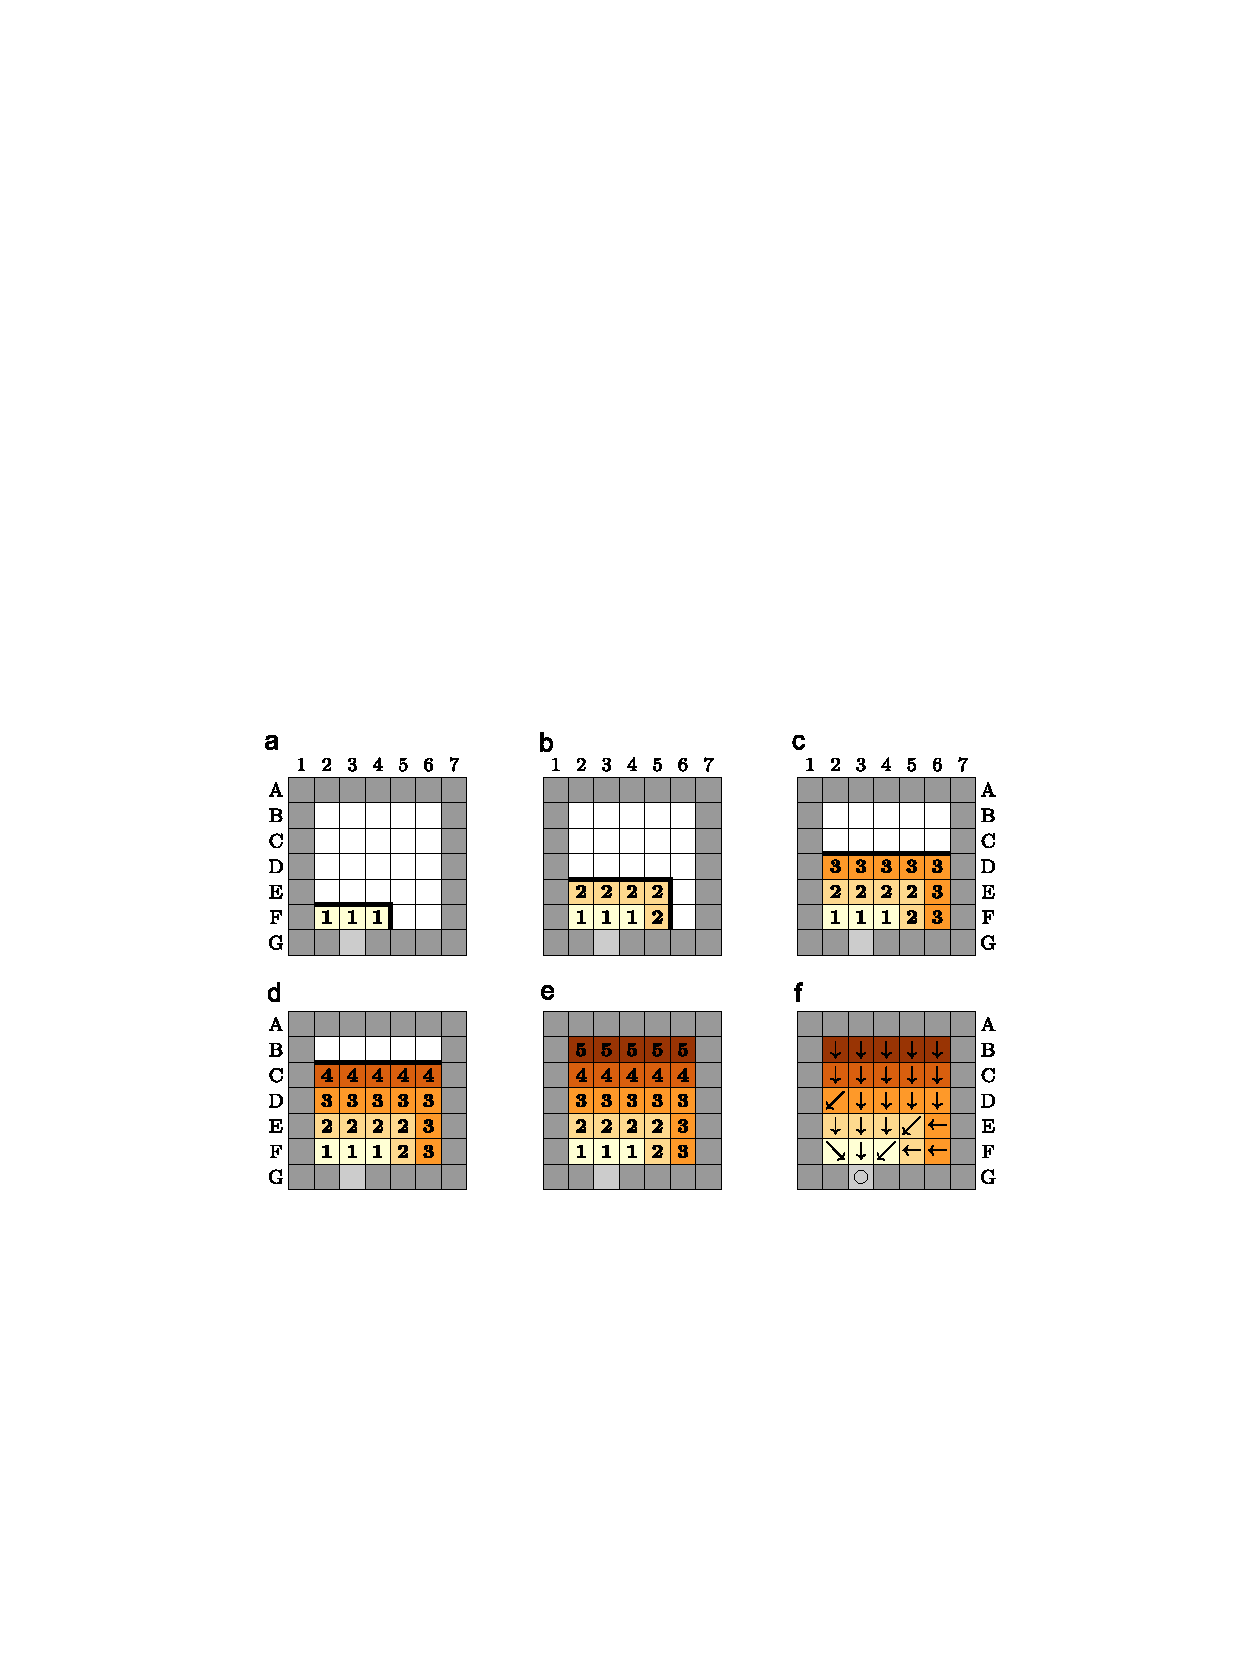
\includegraphics[width=1.0\linewidth]{figs/lt.pdf}
\caption{In a flat surrounded by higher terrain (dark grey) with a single lower-elevation outlet (light grey), we can use a gradient towards from the outlet to route water out of the flat and towards the outlet.
For this, we can iteratively assign (tiny or symbolic) elevation increases in the flat starting from the outlet until all non-draining cells in the flat have been covered.
Figure from \citet{Barnes14}.}%
\label{fig:lt}
\end{figure}


\section{Drainage networks and basins}[Drainage networks]%
\label{sec:drainage_basins}


Interpreting DTM cells as nodes and the flow direction as directed edges connecting them yields the \emph{drainage network}\marginnote{drainage network}\index{drainage network} of a DTM\@.
However, it is usually best to filter out the least important parts of the network using a flow accumulation threshold.
A good rule of thumb for this threshold is the mean flow accumulation in the DTM, but an exact value is usually set by trial and error until the desired parts of the network are kept.

Based on a computed drainage network, it is then possible to extract the \emph{drainage basins}\marginnote{drainage basin}\index{drainage basin}\index{basin} of a DTM by considering the areas that are drained by one or more nodes of the network (Figure~\ref{fig:oceans}).
This operation can be performed in many different places, such as the end node of a river (yielding its river basin), the nodes just before junctions in the network (yielding the drainage basins of the tributaries of a river), or the end nodes of a selected part of the network (yielding the drainage basin of a sea or ocean).
The lines that separate adjacent drainage basins are \emph{drainage divides}\marginnote{drainage divide}\index{drainage divide}, which form topographical ridges.

\begin{figure}[htbp]
\centering
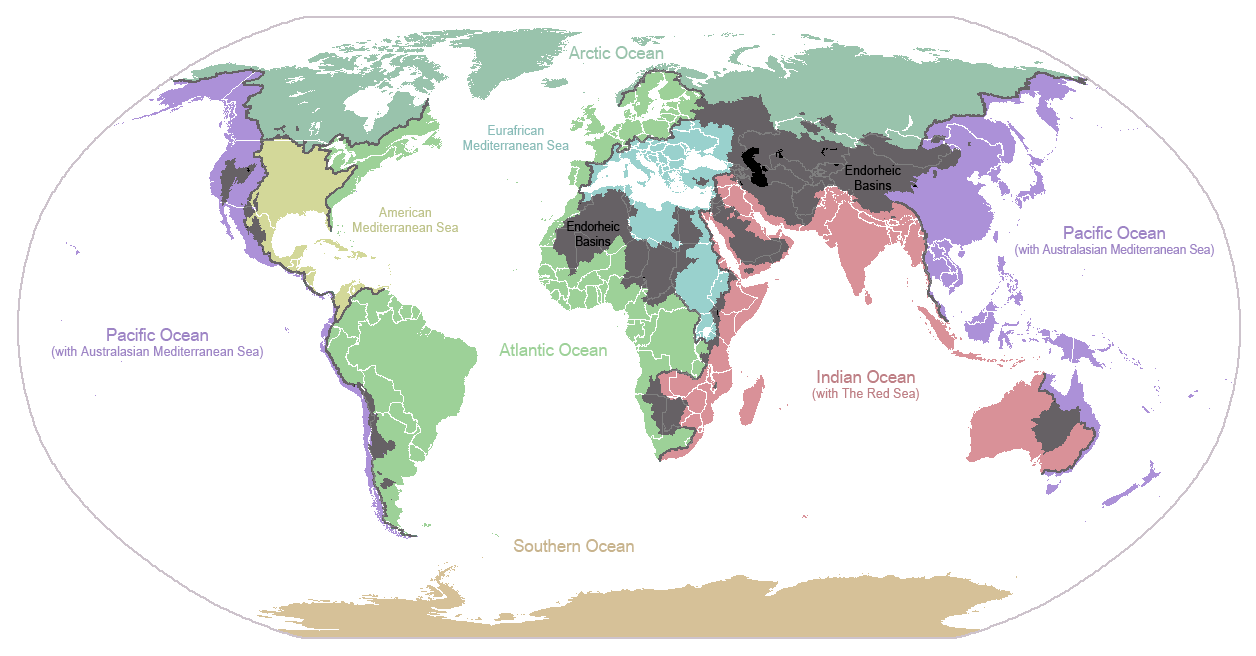
\includegraphics[width=\linewidth]{figs/Ocean_drainage}
\caption{The areas that drain to all the oceans can be computed by selecting the DTM cells on the coastline of these oceans and finding the areas that drain through them.
Note the endorheic basins that drain to none of these cells.
These actually form sinks in the DTM\@.
From Wikimedia Commons.}%
\label{fig:oceans}
\end{figure}

%%%
%
\section{Notes and comments}

\citet{Beven12} is a good reference book on hydrology.
It covers how to make much more complex runoff models than the ones described here.

\citet{OCallaghan84} was the original paper to describe the D8 method.
\citet{Fairfield91} modify D8 into the stochastic rho8 method.
\citet{Quinn91} describes the original MFD method.
\citet{Tarborton97} describes the alternative (D\(^{\infty}\)) MFD method and contains nice figures comparing multiple methods.

\citet{Barnes14a} describes how to fill in sinks, while \citet{Metz11} describes how to use a variation of \(A^{*}\) search algorithm to route water out of them.
\citet{Barnes14} describes how to assign the drainage direction over flats.

%%%
%
\section{Exercises}

\begin{enumerate}
\item Given a raster map of precipitation values, how would you be able to improve the flow accumulation estimates?
\item Why is the flow width important?
\item You have a cycle in your drainage network. How can that happen? How would you solve it?
\item How can you detect endorheic basins without finding all other basins first?
\item Come up with an algorithm to identify flats in a DTM\@.
\end{enumerate}
